\documentclass[spanish,notitlepage,letterpaper, 12pt]{article}
\usepackage[spanish]{babel} 
\usepackage{amsmath}
\usepackage{amsfonts}
\usepackage{amssymb}
\usepackage{graphicx}
\usepackage{geometry}      
\geometry{letterpaper}                  
\usepackage{epstopdf}
\usepackage{fancyhdr} % Paquete para encabezados y pies de pag
\usepackage{listings}
\usepackage{color}
\usepackage{placeins}
\usepackage{csquotes}
\usepackage{textcomp}
\usepackage{gensymb}

\pagestyle{fancy}
\chead{\bfseries Informe 2 - Grupo C1B. Subgrupo 2} 
\rhead{4 de Mayo de 2023}
\cfoot{Universidad Industrial de Santander} 
\rfoot{\thepage} 

\voffset = -0.25in 
\textheight = 8.0in 
\textwidth = 6.5in
\oddsidemargin = 0.in
\headheight = 20pt 
\headwidth = 6.5in
\renewcommand{\headrulewidth}{0.5pt}
\renewcommand{\footrulewidth}{0,5pt}
\begin{document}
\begin{titlepage}
    \begin{center}
        
\includegraphics[width=0.4\textwidth]{../general-images/uis-logo.png}
        
        \vspace{0.5cm}
        \LARGE
        \textbf{Estudio del comportamiento del circuito RLC y el fenómeno de resonancia}
        
        \vspace{0.5cm}
        \large
        Informe 4
        
        \vfill
        
        \textbf{Daniel Esteban Vargas Reyes.} Estudiante - Geología\\
        \textbf{Nicolás Andrés Ramírez Calderón.} Estudiante - Ingeniería de Sistemas\\ 
        \textbf{Rodolfo Valentín Muñoz Vega.} Estudiante - Ingeniería Química\\

        \vspace{1.0cm}
        Presentado a la docente:
        
        \textbf{Zayda Paola Reyes Quijano}
        
        \vfill
        
        Escuela de Física - Física III\\
        Universidad Industrial de Santander\\
        Bucaramanga, Santander, Colombia\\
        20 de Mayo de 2023        
    \end{center}
\end{titlepage}

\tableofcontents

\newpage

\section{Resumen}
Para el siguiente informe se busca explicar de una manera clara el desarrollo de la práctica de laboratorio “Estudio del MAS del Sistema Masa-Resorte y Análisis de las Oscilaciones con CASSY-M”; la cual discierne en la toma de datos para encontrar el valores de elongación y periodo variando la masa para luego tener en cuenta la constante de elongación que se produce al momento de realizar el proceso experimental, además de esto, afianzar los conocimientos del movimiento armónico simple en un sistema masa resorte y sus connotaciones teórico-prácticas que son determinantes para tomar conclusiones acertadas. 

\section{Introducción}
Para entender la naturaleza de los fenómenos oscilatorios, se hace necesario analizar el caso más sencillo, el movimiento armónico simple (MAS) del sistema masa resorte. Este hecho conduce a preguntarse qué factores se involucran en la descripción de las oscilaciones armónicas de un sistema masa-resorte. 

Un sistema masa-resorte es aquel en el que una masa $m$ está anclada al final de un resorte. En un modelo sin ningún tipo de fricción este sistema es útil para representar un movimiento armónico simple (MAS). \cite{serway_jewett_2017}\par
\bigskip
En este proyecto de investigación se estudiarán el período en función de la variación de la masa anclada al resorte y el análisis de las funciones de amplitud, velocidad y aceleración del movimiento.
\subsection{Marco teórico} \label{I.MT}
Un modelo clásico para el análisis del movimiento oscilatorio es el sistema masa resorte en condiciones ideales. Cuando un cuerpo está unido a un resorte y el resorte es deformado una distancia $x$ de su posición de equilibrio, el resorte ejerce una fuerza de magnitud igual a la fuerza que generó su deformación, pero de sentido contrario, pues trata de volver el resorte a la posición de equilibrio. Esta fuerza está dada por la ley de Hooke: 
\begin{align}\label{eq:1}
    \vec{F}=-kx
\end{align}
Donde $k$ es la constante restauradora del resorte y $\vec{F}$ es la fuerza de recuperación que busca traer al resorte de vuelta a su posición de equilibrio. Si un sistema está sometido a una fuerza restauradora, su movimiento es ármonico simple. Al aplicar la segunda ley de Netwon se tiene:
\begin{align}
    \frac{d^2x}{dt^2}=\frac{kx}{m}
\end{align}
Conociendo que la frecuencia angular es $\omega^2=\frac{k}{m}$ la ecuación puede reescribirse de la forma.
\begin{align}
    \frac{d^2x}{dt^2}=-\omega^2x
\end{align}
La función $x(t)$ que satisface la ecuación diferencial dada es: 
\begin{align}\label{eq:2}
    x(t)=A\cos{(\omega t + \varphi)}
\end{align}
Donde $A$, $\omega$ y $\varphi$ representan la amplitud, la frecuencia angular y el ángulo de desfase respectivamente. Lo que esta solución nos dice es que la posición con respecto a la posición de equilibrio de la masa $m$ acoplada al resorte puede estudiarse conociendo las variables
mencionadas.\par
\bigskip
Por otra parte, el tiempo que tarda la masa en completar una osilación completa o \textbf{periodo} $T$ esta dado por: 
\begin{align}
    \label{eq:3}
    T=2\pi\sqrt{\frac{m}{k}}
\end{align}
La ecuación \eqref{eq:3} es la que más utiilidad nos provee para el desarrollo de este laboratorio.
\section{Metodología}
El desarrollo del experimento se realizó en cuatro etapas; tres de observación y obtención de datos y una de análisis de los resultados obtenidos.
\subsection{Materiales}
\begin{enumerate}
    \item Porta pesas.
    \item Juego de pesas.
    \item Soporte universal.
    \item Equipo de cómputo.
    \item Electro-imán.
    \item Cables de conexión.
\end{enumerate}
\subsection{Fase 1} \label{M.F1}
El propósito de esta fase fue corroborar la ley de Hooke. Para ello, fue necesario realizar el montaje experimental (Fig. \ref{Figura 1}), posteriormente se acoplaron diferentes masas, estableciendo la deformación de cada una de ellas sobre el resorte utilizado. Se siguieron los pasos descritos a continuación:
\begin{enumerate}
    \item Se tomaron diferentes masas para producir una deformación sobre el resorte, en concreto masas de 5, 10 y 20 gramos.
    \item Con la ayuda del software CASSY Lab se determinó la deformación producida por cada una de las masas sobre el resorte.
    \item Se registraron los datos en la tabla 1 de la hoja de datos.
\end{enumerate}
\begin{figure}[h]
    \centering
    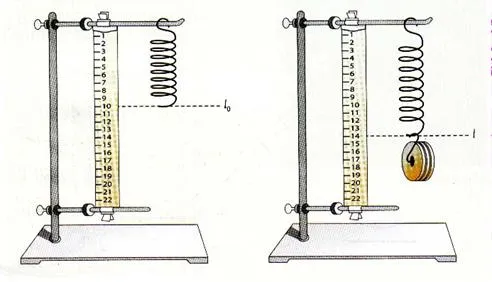
\includegraphics[width=10.0cm]{images/I_MontajeMasaResorte.png}
    \caption{\textit{Montaje experimental sistema masa-resorte}}
    \label{Figura 1}
\end{figure}
\subsection{Fase 2} \label{M.F2}
Con el objetivo de analizar la relación entre la masa $m$ y el periodo de movimiento del sistema $T$ se siguieron estos pasos:
\begin{enumerate}
    \item Se ajustó una configuración de masas (Ej. 10g) en reposo. Y se configuró dicha elongación como la posición de equilibrio en el software CASSY Lab.
    \item Con ayuda de un electroimán se aplicó una fuerza que desplazó la masa de la posición de equilibrió una distancia constante $l$.
    \item Con ayuda de CASSY Lab se soltó la masa en un $t=0$ desde el cual este mismo software midió las oscilaciones por unidad de tiempo, es decir el periodo $T$.
    \item Se registraron los datos en la tabla 1 de la hoja de datos.
    \item Se repitieron los pasos anteriores para todas las configuraciones posibles de masa.
\end{enumerate}
\subsection{Fase 3} \label{M.F3}
Para el análisis de las funciones de amplitud, velocidad y aceleración de un sistema masa-resorte en condiciones reales de nuevo se hizo uso del software CASSY Lab, ya que esta interfaz permite obtener de manera automática numerosos valores precisos de las funciones de movimiento: desplazamiento $s(t)$, velocidad $v(t)$ y aceleración $a(t)$ de la masa acoplada a un resorte que oscila libremente sujeta a la fricción del aire, observándose un movimiento débilmente amortiguado. Los datos fueron guardados en un archivo tipo texto (.txt). 
\subsection{Fase 4}
Haciendo uso de los datos obtenidos en las fases anteiores se realizó un tratamiento y un análisis de los fenómenos estudiados.\par
\bigskip
De la fase \ref{M.F1} se determinó la relación entre la fuerza y la deformación del resorte con el objetivo de corroborar la ley de Hooke. Con los datos de la fase \ref{M.F2} se analizó la relación entre la masa y el periodo del sistema masa resorte determinando la constante restauradora del resorte
a partir de la ecuación \eqref{eq:3}. En el caso de la fase \ref{M.F3} se realizó el análisis de las funciones de movimiento $s(t)$, $v(t)$ y $a(t)$ del sistema masa resorte en condiciones reales mediante las ecuaciones de estas funciones y los elementos que definen este movimiento, tales como el
período, la amplitud, la constante de amortiguamiento, el desfase entre la amplitud, la velocidad y la aceleración, entre otros.\par
\bigskip
Para todos los casos el estudio se apoyó en un análisis gráfico de los datos sustraidos durante la parte experimental del laboratorio. 
\section{Tratamiento de datos} \label{TD}
El movimiento armónico simple es aquel que describe un objeto el cual se somete a una fuerza restauradora que para nuestro caso se representa como la constante del resorte $k$ proporcional al movimiento, dicho de otra manera, se genera un movimiento periódico representado de manera gráfica por medio
de unas ondas mostrando dichas oscilaciones con respecto al tiempo; ciertas características permiten afirmar que se trata de este movimiento, ya que no tiene amortiguación, sabiendo que la fuerza recuperadora cumple la función de conservar la energía descrita como el cambio de energía potencial a
cinética y viceversa con la finalidad de buscar el equilibrio, asimismo, la ausencia del rozamiento permite sustentar lo descrito anteriormente. Por otra parte, la magnitud de la amplitud y el periodo se mantienen constantes a través del tiempo, puesto que no existe un factor externo que afecte el
tipo de movimiento presentado.\par
\bigskip
Debemos tener en cuenta la ley de Hooke \eqref{eq:1}.\par
\bigskip
Planteamos una relación a una función lineal de la forma $mx + b$, vemos que presenta cieta analogía puesto que la constante $K$ se va a representar la dependencia de dicha recta, la cual no ofrece un corte con el eje $Y$ para los datos que tenemos con referencia, por medio de los siguientes datos
tabulados se plantea que el peso representado como el producto entre la masa y la gravedad en función de la deformación, nos generará el valor de la fuerza restauradora.
\begin{table}[h]
    \centering
    \begin{tabular}{l|c|c|l}
        Masa $[Kg]$ & Peso $[N]$ & Elongación $[m]$ & Periodo $[s]$ \\
        \hline \hline
        $0$ & $0$ & $0$ & $0.875$\\
        $0.005$ & $0.049$ & $0.017$ & $0.917$\\
        $0.010$ & $0.098$ & $0.032$ & $0.949$\\
        $0.015$ & $0.147$ & $0.049$ & $0.985$\\
        $0.020$ & $0.196$ & $0.065$ & $1.017$\\
        $0.025$ & $0.245$ & $0.082$ & $1.048$\\
        $0.030$ & $0.294$ & $0.097$ & $1.078$\\
        $0.035$ & $0.343$ & $0.114$ & $1.108$\\
    \end{tabular}
    \caption{\textit{Registro del periodo y la elongación en función del cambio de la masa}}
    \label{Table 1}
\end{table}
En el gráfico (Fig. \ref{Figura 2}) se evidencia que el valor de $k$ es $3.0172 \ [N/m]$
\newpage
\begin{figure}[ht]
    \centering
    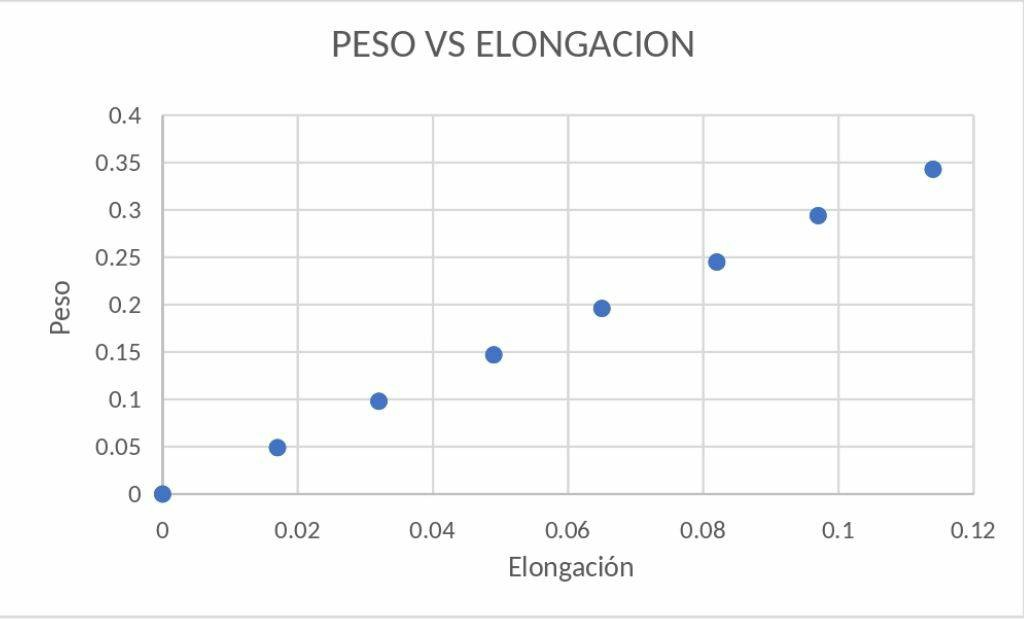
\includegraphics[width=10.0cm]{images/peso-vs-elongacion.png}
    \caption{\textit{Análisis del peso vs la elongación}}
    \label{Figura 2}
\end{figure}
Es posible presentar otro tipo de análisis con respecto a los datos descritos en la siguiente tabla, pero para este caso se tiene en cuenta la ecuación diferencial de segundo órden. \eqref{eq:2}\par
\bigskip
También contamos con otras dos características más expresadas como periodo, el cual esta definido como el tiempo necesario para realizar una oscilación y la frecuencia interpretada de acuerdo con el número de vibraciones completas por unidad de tiempo, hallada tras determinar la segunda derivada de
la posición con respecto al tiempo. En este punto se hace uso de la fórmula de periodo vista anteriormente. \eqref{eq:3}\par
\bigskip
Al utilizar los datos arrojados por el sistema Cassy-lab en donde posteriormente se genera una gráfica del periodo al cuadrado con respecto a la masa con el fin de despejar la constaste restauradora del resorte que, en su defecto, coincide con el valor de la pendiente de la gráfica (Fig. \ref{Figura
3}), puesto que, en teoría según la ley e Hooke existe una dependencia de la constante del periodo con respecto a la masa.
\newpage
\begin{table}[ht]
    \centering
    \begin{tabular}{l|l}
        Masa $[Kg]$ & Periodo cuadrado $[s^2]$ \\
        \hline \hline
        $0$ & $0.765625$ \\
        $0.005$ & $0.840889$ \\
        $0.010$ & $0.900601$ \\
        $0.015$ & $0.970225$ \\
        $0.020$ & $1$ \\
        $0.025$ & $1.09$ \\
        $0.030$ & $1.16$ \\
        $0.035$ & $1.22$ \\
    \end{tabular}
    \caption{\textit{Registro del periodo al cuadrado en función del cambio de la masa}}
    \label{Table 2}
\end{table}
Entonces, al analizar la información registrada en la tabla (Cdr. \ref{Table 2}) se obtiene una recta creciente (\ref{Figura 3}).
\begin{figure}[ht]
    \centering
    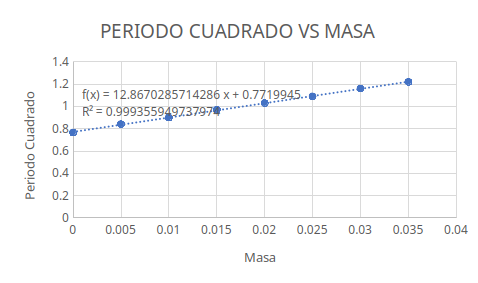
\includegraphics[width=10.0cm]{images/periodo-cuadrado-vs-masa.png}
    \caption{\textit{Análisis el periodo al cuadrado vs la masa}}
    \label{Figura 3}
\end{figure}
\\
Teniendo en cuenta el valor de pendiente representado en la gráfica (Fig. \ref{Figura 3}) la cual equivale a $0.772$ se tiene que la constante $k$ evaluando la fórmula $k=\frac{4\pi^2}{m}$ es igual a:
\begin{align*}
    k=\frac{4\pi^2}{12.867}\\
    k=3.0681 \ [N/m]\\
\end{align*}
Por último, para la última fase se cuenta con tres tablas de datos las cuales generan diferentes gráficas con una masa constante de $35 \ g$, en donde se relacionan magnitudes físicas propias del movimiento armónico amortiguado libre (M.A.A.L) reconocidas como: velocidad, recorrido y aceleración con
respecto al tiempo; por otro lado, para una elongación equivalente a TARDIGRADO 1 (obtenido de la aplicación Cassy-lab) se tiene un movimiento oscilatorio representado por medio de ondas como se puede observar en la gráfica (Fig. \ref{Figura 4}).
\begin{figure}[ht]
    \centering
    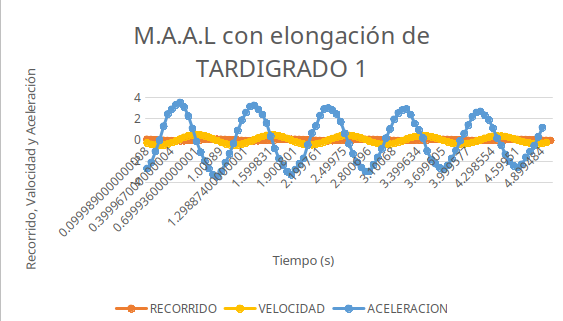
\includegraphics[width=10.0cm]{images/tardigrado1.png}
    \caption{\textit{Recorrido, velocidad y aceleración en función del tiempo con elongación TARDIGRADO 1.}}
    \label{Figura 4}
\end{figure}
\bigskip
Asimismo, para una elongación de TARDIGRADO 2, se considera otro gráfico alusivo a los datos muestreados. (Fig. \ref{Figura 5})
\begin{figure}[h]
    \centering
    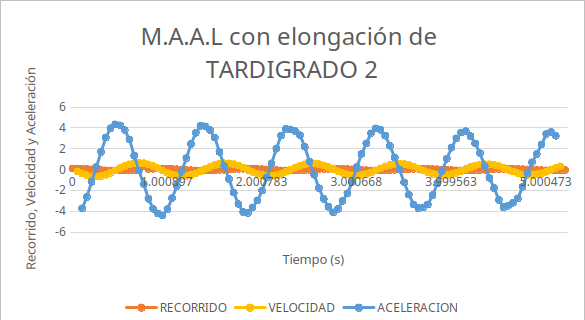
\includegraphics[width=10.0cm]{images/tardigrado2.png}
    \caption{\textit{Recorrido, velocidad y aceleración en función del tiempo con elongación TARDIGRADO 2.}}
    \label{Figura 5}
\end{figure}
\bigskip
Con una elongación correspondiente a TARDIGRADO 3, se tiene otro gráfico ropio del M.A.A.L (Fig. \ref{Figura 6}), en donde ocurren ciertas variaciones con respecto al M.A.S que se analizarán posteriormente.
\newpage
\begin{figure}[ht]
    \centering
    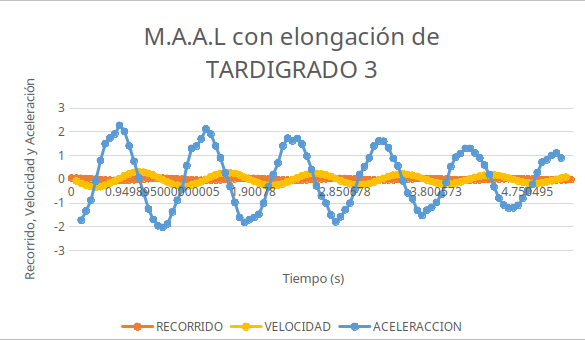
\includegraphics[width=10.0cm]{images/tardigrado3.png}
    \caption{\textit{Recorrido, velocidad y aceleración en función del tiempo con elongación TARDIGRADO 3.}}
    \label{Figura 6}
\end{figure}
Finalmente se toman las amplitudes mas altas en las graficas anteriores y se realiza la respectiva linealización en este caso con una función exponencial para encontrar así el coeficiente de amortiguamiento.
\begin{figure}[ht]
    \centering
    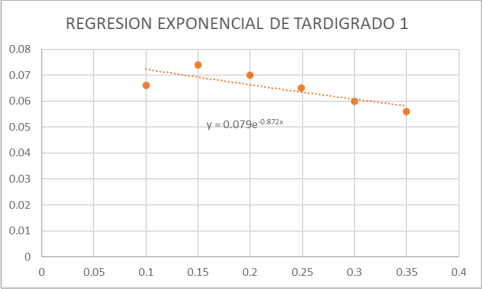
\includegraphics[width=10.0cm]{images/regresion-tardigrado1.png}
    \caption{\textit{Regresión exponencial de TARDIGRADO 1.}}
    \label{Figura 7}
\end{figure}
\bigskip
En la regresión de TARDIGRADO 1 (Fig. \ref{Figura 7}) se evidencia un $\gamma=0.872$ de coeficiente de amortiguamiento.
\newpage
\begin{figure}[ht]
    \centering
    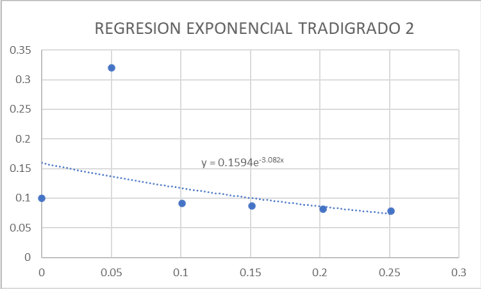
\includegraphics[width=10.0cm]{images/regresion-tardigrado2.png}
    \caption{\textit{Regresión exponencial de TARDIGRADO 2.}}
    \label{Figura 8}
\end{figure}
La regresión de TARDIGRADO 2 (Fig. \ref{Figura 8}) contempla un $\gamma=0.1594$ de coeficiente de amortiguamiento.
\begin{figure}[ht]
    \centering
    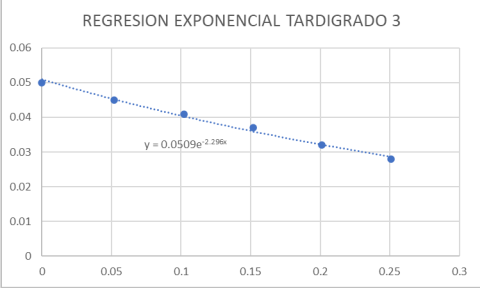
\includegraphics[width=10.0cm]{images/regresion-tardigrado3.png}
    \caption{\textit{Regresión exponencial de TARDIGRADO 3.}}
    \label{Figura 9}
\end{figure}
\bigskip
En el caso de TARDIGRADO 3 (Fig. \ref{Figura 9}) se hace claro un $\gamma=0.0509$ de coeficiente de amortiguamiento.
\section{Análisis de resultados}
Inicialmente en el proceso de toma de datos, se esperaban ciertos resultados, con los cuales objetivamente se compararían con los tomados en el proceso experimental. Como se esperaba en el grupo de trabajo; a medida que se da una mayor masa al resorte, este tiene una mayor elongación, y esto se
puede apreciar en la gráfica que las relaciona (Fig. \ref{Figura 2}), donde se ve un crecimiento en el peso y en la elongación de manera directa. Tambien se puede decir que el gráfico, ciertamente obedece la ley de hooke, teniendo en cuenta todo esto, se pudo hallar el valor de la constante $k$.\par
\bigskip
Por otra parte, referente al simulador Cassy-lab, se trabajó con una masa de valor constante, se obtuvieron graficos donde se ve evidenciado como se relaciona, el recorrido, la velocidad y la aceleración, respresentadas por curvas sinosoidales, y en retrospectiva, haciendo una comparación con los resultados que esperabamos, se acercan mucho.
\section{Conclusiones}
Cerrando con el proceso de experimentación y de investigación, se pudieron cumplir los objetivos previstos, se lograron entender los diferentes fenómenos físicos que actúan en un M.A.S en sistema masa-resorte, tal como se esperaba.\par
\bigskip
Se trabajaron con diferentes valores de masas para ver como actuaba
el sistema y cuáles eran sus cambios, estos fueron observados y sus datos tomados y recopilados, haciendo un análisis de estos, y llegando a una conclusión de que el aumentar la amplitud se evidencia que la masa viaja una mayor distancia durante un ciclo. Sin embargo, incrementar la amplitud también
aumenta la fuerza de restitución, este aumento en la fuerza incrementa proporcionalmente la aceleración de la masa, por lo que la masa se mueve una mayor distancia en el mismo tiempo. Así que aumentar la amplitud no tiene un efecto neto en el periodo de la oscilación.\par
\bigskip
Por último, también se cumplió el objetivo principal el cual era conocer cómo funciona un MAS en sistema masa-resorte.
\section{Referencias} 
\bibliographystyle{unsrt}
\bibliography{../general-references/references}
\end{document}
